\section{Gestion de flux de données}\label{sec:rw:supervision:datastream}
Devant la multiplication des applications à base de flux de données telles que : la gestion des données de capteurs ou la surveillance réseau, les systèmes de gestions de flux de données (\textit{SGFD}) ont étés conçus pour mieux maîtriser les données de ce types de systèmes~\cite{Madden:tag, Yao:cougar, Cranor:gigascope}. L'idée principale de ce type de système étant de permettre une utilisation des flux de données de la même manière que les bases de données. L'interrogation des flux passerait donc par un langage déclaratif (tout comme le \textit{SQL}) avec un grand pouvoir d'expression.

La gestion de flux est le socle fondamental des systèmes capables de traiter les événements. Les travaux récents sur les \textit{CEP} (\textit{Complex Event Processing}) permettant de faire de la détection d'événement complexe~\cite{Brenna:cayuga} est au final une extension des SGFD avec des opérateurs spécifiques et optimisés.
\subsection{Approche des SGFD}
Un flux de données est une série continue et ordonnée de données qui s'accumule au fur et à mesure du temps~\cite{Golab:issues}. De façon générale, il n'est pas supposé une régularité temporelle sur l'arrivée des données dans le flux (tel que \enquote{\it une donnée toutes les 5 secondes}). L'idée de faire une interrogation sur ces flux de données au sens \enquote{gestion de base de données} du terme n'a pas de sens car il y aurait confusion entre les modes d'interrogations continues et instantanées présentés en section~\ref{sec:rw:supervision:criteres:traitement}. En effet, le paradigme des requêtes est fondamentalement différent car les requêtes sont de longue durée et persistantes~\cite{Chen:niagaracq}.
\begin{figure}[ht]
    \centering
    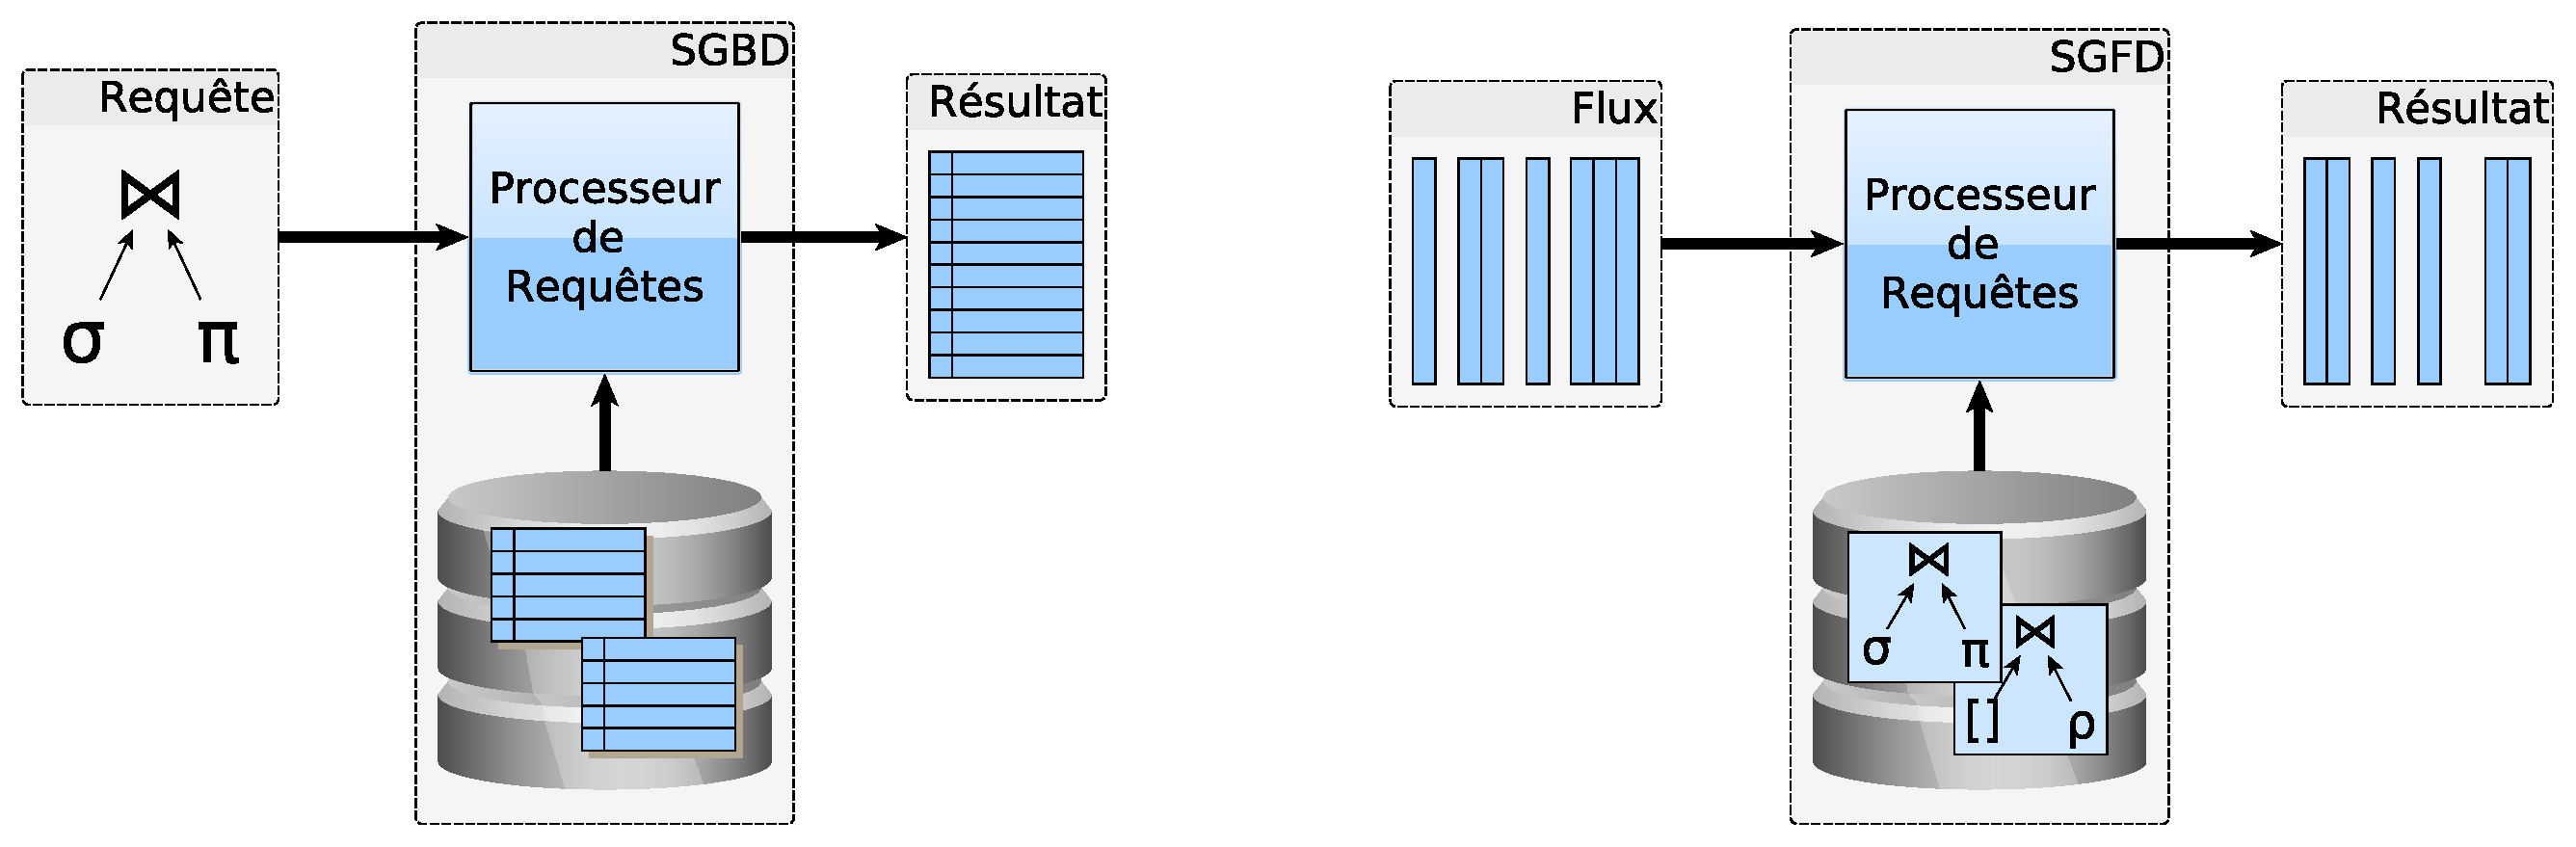
\includegraphics[width=0.75\textwidth]{rw-supervision-sgbd-sgfd}
    \caption{SGBD : Requêtes transitoires, Données persistantes vs SGFD : Données transitoires, Requêtes persistantes~\protect\cite{Gurgen:sstreamware}}
\end{figure}

\begin{itemize}
    \item[\textbf{Base de données}] : Une requête est une question posée sur un ensemble de relations figées et persistants (principe transactionnel). La réponse est un ensemble de n-uplets. Une fois la requête traitée elle n'existe plus.
    \item[\textbf{Flux de données}] : Une requête un ensemble d'opérateurs et est considéré comme persistant. Le ou les flux de données sont appliqués sur cet ensemble d'opérateurs pour en produire un nouveau flux. La particularité d'un flux de données étant qu'une fois la donnée \textit{consommée}, elle n'est plus considéré comme présente dans le flux d'entrée. Les données fournies en entrée de la requête sont donc transitoires.
\end{itemize}

Ainsi, le terme \textit{requête} a un tout autre sens. Toutefois, beaucoup de concepts sont applicables dans ce contexte. En effet, plusieurs éléments de modélisation issues du relationnel sont appliqués dans ce domaine~\cite{Arasu:semantic}. Historiquement, les premières requêtes continues~\cite{Terry:tapestry} étaient une exécution périodique de requêtes \textit{SQL}. Le traitement était entièrement basé sur les opérateurs du modèle relationnel standard. Par la suite, les modèles ont évolués pour supporter nativement le dynamisme des données.

\subsection{Principes architecturaux}
L'architecture abstraite d'une solution de gestion de flux de données est composés de trois parties principales~\cite{Duller:virtualdsms}.
\begin{itemize}
 \item[\textbf{Les sources}] : Ces composants permettent d'abstraire une source de données dans le formalisme du SGFD. Ce composant produit donc un \textit{flux} ou tout autre entité dynamique du système. Par exemple, ceci peut être un composant capable de dialoguer dans un protocole donné pour collecter des informations brutes sur un équipement. Il est important de noter que \textbf{la source contrôle le dynamisme} a priori. En effet, dans un \textit{SGFD} la source de données décide du moment où va être envoyé une donnée. Donc, si une information n'est accessible que par une sonde dont le mécanisme est en \textit{pull} par exemple, la source devra interroger cette sonde périodiquement (ou à date fixé). Le choix de cette période (ou de cet instant) dépendra de son implémentation.
 \item[\textbf{Le processeur}] : Cet ensemble est le cœur du \textit{SGFD}. Il va traiter les entités fournies par les différentes sources de données qui lui sont données. En sortie, il produit une nouvelle entité. Le processeur est composés d'opérateurs ainsi que de composants pour gérer son cycle de vie et son exécution (\textit{planificateurs}, \textit{gestionnaires de ressources}).
 \item[\textbf{Le puit}] : Ce composant fait l'interface entre l'application utilisatrice du \textit{SGFD} et le résultat de requête. Il permet de transférer les résultats selon un format ou un mécanisme en particulier.
\end{itemize}
Bien évidemment, des gestionnaires globaux permettant de répertorier les sources, lister les différentes requêtes déployées, et évidemment de contrôler les requêtes peuvent être définis pour interagir avec le système. Il est important de noter que l'approche initiale des \textit{SGFD} est de pouvoir interagir avec le système dans un langage déclaratif. Des extensions de \textit{SQL} ont vu le jour~\cite{Arasu:cql, Chandrasekaran:telegraphcq} pour remplir cette tâche. Toutefois, devant la large complexité des requêtes, certains travaux ont préféré définir des langages procéduraux où la composition des opérateurs doit se faire à la main~\cite{Abadi:aurora, Gurgen:sstreamware}, de façon graphique ou textuelle.

Comme présenté, le processeur est composé de multiples opérateurs. De la même façon qu'en gestion de base de données, une requête est au final un arbre d'opérateur\footnote{Dans la pratique, dans un SGFD, il est courant de plutôt trouver des graphes directs acycliques dû à la mutualisation de sous-parties de requêtes. La mise à l'échelle des requêtes de longévité indéterminé fait qu'il est important de ne pas dupliquer les sous-résultats. Toutefois, d'une manière conceptuelle, il reste juste de dire qu'une requête est formé d'un arbre.}.
Afin de supporter le dynamisme inhérent aux entités, plusieurs nouveaux opérateurs ont étés développés.

\subsection{Les opérateurs}
Les opérateurs sont souvent classés en deux catégories : les bloquants et non-bloquants. La particularité des opérateurs bloquants est de ne pas être exécuté à chaque donnée reçue. Contrairement aux systèmes événementiels où les événements sont traités à réception, les opérateurs bloquant ont leurs propre cycle de vie.
\subsubsection{Fenêtres}
L'opérateur blocant le plus répandu reste avant tout l'opérateur de fenêtrage. Le principe étant de regrouper des données du flux selon un critère temporel ou positionnel, comme les \textit{5 dernières minutes} ou \textit{les 10 dernières valeures}. Ceci permet de considérer le flux comme un ensemble et non comme un suite de données décorrélé.

Lors de la description des types de dynamismes en section~\ref{sec:intro:problematique:data}, le concept de régularité a été exposé. L'importance et la plus-value qu'il est possible d'extraire de ces données se base sur le fait de pouvoir en regrouper plusieurs et analyser cet ensemble. C'est pour cela que l'opérateur de fenêtre a longtemps été utilisé avant tout et seulement pour l'agrégation de données~\cite{Madden:tag, Abadi:aurora}. En combinant un opérateur de fenêtre et un opérateur capable de calculer une moyenne, il est possible de calculer la requête \enquote{\it Flux des moyenne de température sur 5 minutes du capteur 42}. Cette combinaison d'opérateur est celle utilisée récemment dans les SGBD relationnels. En effet, la norme \verb|SQL:2003| a introduit l'opérateur explicite \verb|WINDOW| qui s'applique sur un agrégat.

Toutefois, la complexité de la sémantique dû à son indépendance a mené les travaux de recherche à de multiples définitions parfois conflictuelles~\cite{Jain:spread}. Car, l'évolution des bornes est certes une caractéristique à prendre en compte, mais le taux de rafraîchissement de l'opérateur (\textit{toutes les 2 minutes}, \textit{toutes les 10 données}) implique aussi un contrôle difficile. Notons qu'une fenêtre avec un taux de rafraîchissement différent de la taille de la fenêtre est nommée \enquote{\it glissante}.

Cet opérateur ne se retrouve pas toujours dans les SGFD à l'état naturel car les modèles de données ne supportent pas tous le fait de séparer les fenêtres des autres opérateurs qui en ont besoins.

\subsubsection{Les jointures de flux}
Pour permettre l'intégration de deux flux en un nouveau, il existe deux méthodes principales. L'union, pour chaque n-uplet entrant dans l'un ou l'autre des deux flux, il se retrouvera dans le flux résultant. La deuxième méthode étant de faire une jointure comme il est possible dans le modèle relationnel.

Toutefois, le fait étant qu'un flux n'a pas de représentation relationnelle directe car son nombre de donnée est potentiellement infini. Donc la jointure n'a pas de sens direct. En revanche, les mécanismes du fenêtrage permettent de sélectionner une partie précise et finie du flux à tout moment. Ainsi, les jointures ont permit de faire l'intégration des données.

La jointure se fait donc soit sur l'ensemble des données jusqu'à présent (jointure historique), soit par la dernière donnée connue (jointure présente), soit par égalité des \textit{timestamps} (jointure synchronisée), soit par tolérance temporelle (jointure par bande). La complexité des fenêtrages est donc reportée sur l'opérateur de jointure, cela inclut les ambiguïtés sémantiques observées.

\subsubsection{Performances}
Les opérateurs bloquants ont une complexité très haute dû à leur cycle de vie indépendant. D'un point de vue performance, il est important que les opérateurs soient exécutés le plus rapidement possible. En effet, dans les applications habituellement visée, il est possible d'obtenir des cadences de plusieurs centaines de données par seconde dans les flux. Chaque opérateur doit donc être efficace pour ne pas perturber l'exécution.

Pour mieux supporter les débits, certaines solutions suppriment des données de flux réguliers pour éviter l'encombrement~\cite{Tatbul:load-shedding}. D'autres fournissent des opérateurs capables de calculer des agrégats à la volée de manière approximative~\cite{Babcock:sampling}.

\subsection{Synthèse}
\begin{table}[!ht]
\criteretabDonnee
    {Modèle dérivé du relationnel mais où le contenu est variable dans le temps.}
    {Pas de structure sémantique en dehors de gestion de méta-données ad hoc pour les sources.}
    {Toutes les données sont dynamiques et événementielles a priori.}
\criteretabTraitement
    {Continue.}
    {Il est supposé que chaque source produit un flux de données. Le fait de traiter ces flux participe à l'intégration de sources.}
    {Langages de requêtes similaires aux SQL supportant la dynamique et l'évolution des données}
    {A un instant donné, les opérateurs sont semblables au relationnel. L'expressivité du support du dynamisme reste inconnu encore.}
\criteretabAdaptabilite
    {Création de source pour fournir les flux de données. Comme il n'y a pas de structure sémantique, l'adaptation n'est que l'écriture de requêtes continues.}
    {Pas de perspectives métiers.}
    {Les sources et puits sont en général adaptés par les utilisateurs. Un développement peut être fait dessus, mais il est rarement possible de rajouter des opérateurs.}
    {Très rapide car la latence de traitement doit être contrôlée pour supporter des haut débits.}
\caption{Synthèse des systèmes de gestion de flux de données}\label{tab:rw:supervision:sgfd:synthese}
\end{table}

La gestion de flux de données a été créée pour mieux gérer le dynamisme des données. Le résultat montre qu'effectivement, il est possible de faire des requêtes continues sur des flux de données de manière déclarative et avec une performances très efficace. Toutefois, la complexité qui en ressort comparée à celle de l'algèbre relationelle est plus haute. Beaucoup de systèmes n'ayant pas besoin de cette diversité restreignent leurs opérateurs pour être plus facilement utilisable. L'exemple le plus courant étant le domaine de la gestion de flux d'actualité (\textit{RSS}) où le schéma est constant et l'intégration à base d'union.

Les données sont malgré tout considéré comme volatiles et il n'existe pas de modèle de description pour identifier la sémantique des informations contenues dans les flux. Aucun support de persistence n'existe de manière intégrée. Plusieures approches amènent de la gestion de méta-données voire même des bases complètes mais l'intégration se fait de façon ad-hoc.
